\chapter{The World Needs Changes or Application Customisation}\label{ch00:03}

\myepigraph{Technical skill is mastery of complexity, while creativity is mastery of simplicity.}{Erik Christopher Zeeman}

  Before making any changes to the generated applications, we should discussed its modules, which are typical for any TG-based application project, their roles and interdependencies.

\section{Project Modules}
  The generated application consists of six modules with interdependencies depicted in Fig.~\ref{img:ch00:03:project_module_dependencies}.
  These modules are grouped into three independent groups: Server Modules, Client Modules and Shared Module.
  
  \begin{description}
    \item[\textbf{Shared Module.}] Includes a single module \texttt{coolapp-pojo-bl}, which is independent from other application modules, and is shared between the other two groups.
	This module represents the very core of the application where the business domain model is defined.   
    \item[\textbf{Server Modules.}] Include two modules -- \texttt{coolapp-dao} and \texttt{coolapp-web-server} -- that together define the application web server.	
      \begin{itemize}
	\item \texttt{coolapp-dao} -- contains Data Access Objects (DAO), which are the database-aware implementations of controllers defined as part of the \texttt{coolapp-pojo-bl} module; designed to support domain driven unit testing, which makes it a natural choice for data-oriented unit tests.
	\item \texttt{coolapp-web-server} -- represents an entry point for the server-side application; has a transitive dependency to module \texttt{coolapp-pojo-bl} via a direct dependency to \texttt{coolapp-dao}; registers web resources associated with domain entities, which bind together controllers with their DAO implementations.
      \end{itemize}
    \item[\textbf{Client Modules.}] Include three modules~--~\texttt{coolapp-rao}, \texttt{coolapp-ui} and \texttt{coolapp-web-client}~--~that together define the application web client.
      \begin{itemize}
	\item \texttt{coolapp-rao} -- contains (web) Resource Access Objects (RAO), which are HTTP-aware implementations of controllers defined as part of the \texttt{coolapp-pojo-bl} module, which is its only dependency.
	\item \texttt{coolapp-ui} -- contains User Interface elements such as frames, panels, menu items.
	\item \texttt{coolapp-web-client} -- represents an entry point for the client-side application; has a transitive dependency to module \texttt{coolapp-pojo-bl} via a direct dependency to \texttt{coolapp-rao} and \texttt{coolapp-ui}; binds together controllers defined in \texttt{coolapp-pojo-bl} with their RAO implementation, which ensures resolution of contract dependencies in \texttt{coolapp-ui}.
      \end{itemize}
   \end{description}

\begin{image}{Dependencies between Project Modules.}{\label{img:ch00:03:project_module_dependencies}}    
    \scalebox{1.0} {
  \begin{tikzpicture}
    \draw[very thick, dashed, color=blue!50!black, rounded corners] (-2.3, 1.8) rectangle (10.7,-1.2);
    \node[rotate=90,color=blue!50!black] at (-2.6, 0.25) {\small Server Modules};

    \umlbasiccomponent[x=0, y=0, fill=blue!10]{coolapp-dao}
    \umlbasiccomponent[x=8, y=0, fill=blue!10]{coolapp-web-server}

    \draw[very thick, dashed, color=red!50!black, rounded corners] (1.8, -3.3) rectangle (6.2,-6.1);
    \node[color=red!50!black] at (4.9, -3) {\small Shared Module};
    \umlbasiccomponent[x=4, y=-5]{coolapp-pojo-bl}
    
    \umlnote[x=-2, y=3.5, width=5.5cm, fill=annotationbgcolor]{coolapp-dao}{\scriptsize Date Access Objects layer, which provides RDBMS-based implementation for domain controllers.}
    \umlnote[x=-2, y=-3.5, width=5.5cm, fill=annotationbgcolor]{coolapp-pojo-bl}{\scriptsize Defines business domain model (entities and controllers), shared between client and server tiers.}

    \umluniassoc{coolapp-dao}{coolapp-pojo-bl}
    \umluniassoc[name=w2d]{coolapp-web-server}{coolapp-dao}
    \umlnote[x=5, y=3.5, width=5.5cm, fill=annotationbgcolor]{w2d-1}{\scriptsize Web resources use DB driven implementation of domain controllers} 

    \draw[very thick, dashed, color=green!50!black, rounded corners] (-1, -8.1) rectangle (8.9,-15.2);
    \node[rotate=90,color=green!50!black] at (-1.3, -9.7) {\small Client Modules};

    \umlbasiccomponent[x=7, y=-10, fill=green!30]{coolapp-ui}
    \umlbasiccomponent[x=1, y=-10, fill=green!30]{coolapp-rao}
    \umlbasiccomponent[x=4, y=-14, fill=green!30]{coolapp-web-client}   

    \umlnote[x=-2, y=-6.5, width=5.5cm, fill=annotationbgcolor]{coolapp-rao}{\scriptsize Resource Access Objects, which provides HTTP-based implementation for domain controllers.}
    \umlnote[x=-3, y=-13.7, width=3cm, fill=annotationbgcolor]{coolapp-web-client}{\scriptsize Binds together UI and RAO implementation of domain controllers to define a web client application.}

    \umluniassoc[name=u2m]{coolapp-ui}{coolapp-pojo-bl}
    \umlnote[x=9, y=-6, width=3.5cm, fill=annotationbgcolor]{u2m-1}{\scriptsize Accessed domain model and controller via their contracts (not implementation).} 
    \umluniassoc{coolapp-rao}{coolapp-pojo-bl}
    \umluniassoc{coolapp-web-client}{coolapp-ui}
    \umluniassoc{coolapp-web-client}{coolapp-rao}  

  \end{tikzpicture}
  }
  \end{image}

  The role for each module is well defined and serves as one of the aspects of the TG development model.
  The core value of the application is in its business domain model.
  Module \texttt{coolapp-pojo-bl} is used for defining all domain entity types, validation and controller contracts that model the business domain for which the application is being constructed.
  Each domain entity type is associated with a corresponding CRUD (Create Request Update Delete) controller contract, which serves as the primary way to interact with domain entities.
  The \texttt{coolapp-rao} and \texttt{coolapp-dao} module fulfil client and server side implementation of domain controllers respectively.
  All essential functionality for CRUD controllers is provided by the platform, and is reused by sub-typing corresponding platform classes.\footnote{Later chapters provide all details on how this is done, how to properly reuse and customise provided functionality.}.
  There are guidelines as to what logic is better suited for the client side and what for the server side of the applicaton.
  These are provided in later chapters of this book.  

\section{Quick changes}

  In order to provide a sense of what it is like to change TG-based application let's consider one of the entity types, which is provided as part of the generated application -- \emph{Person} -- listed in Listing~\ref{lst:Person}.

 \lstset{language=Java,
	  escapechar=\%,
	  numbers=left, numberstyle=\tiny, basicstyle=\scriptsize\color{basiccolor}, stepnumber=1, numbersep=5pt, keywordstyle=\bfseries\color{codefgcolor}, stringstyle=\color{stringcolor}}
  \begin{code}{A fragment of entity type Person.}{\label{lst:Person}}{codebgcolor}
    \begin{lstlisting}
@KeyType(String.class)
@KeyTitle(value = "Person Code", desc = "A code uniquely representing a person.")
@DescTitle(value = "Description", desc = "A short description...")
@MapEntityTo("CRAFT")
@DefaultController(IPerson.class)
public class Person extends AbstractEntity<String> {
    .....................
    @IsProperty
    @Title(value = "Username", desc = "Application user name")
    @MapTo("USER_NAME")
    private String username;
    .....................
}
    \end{lstlisting}
  \end{code}
  
  The purpose of entity Person is to model a concept of a person that is either using the application or needs referenced by any other domain entity, which might be required by some business process implemented in the application.
  The platform provides a concept of the application user, which is implemented by entity \emph{User}.
  This entity is an integral part of the platform and cannot be changed in any derived application\footnote{More detailed on entity User is provided as part of security related chapter.}.
  The Person entity reuses this User concept by sharing some of its properties.
  Specifically, property \emph{username} and \emph{password}.
  This way Person and User fuse together, which is not required, but convenient.  

\subsection{Attributes for Entity and its Properties}
  Any custom Java type that subtypes \emph{AbstractEntity} is an entity from platform perspective.
  Type AbstractEntity is very rich in its functionality and provides full support for modeling a wide variety of business domain entities.
  It is discussed in great details further in the book.
  So, here we just touch on some of the aspects of domain entity modeling.

  Domain entities may have \emph{simple} or \emph{composite} (more than property is involved) business key, which uniquely identifies each entity instance.
  Entity Person has a simple business key of type String, which is specified by annotation \emph{KeyType}  and \emph{AbstractEnity} type parameter as can be observed in Listing~\ref{lst:Person} at lines 1 and 6.
  
  Each property of domain entities can be provided with a user friendly title and description, which is used by the system when building UI or reporting warnings/errors.
  This is done by annotating property representing fields with annotation \emph{Title} such as depicted in Listing~\ref{lst:Person} at line 9.
  However, property \emph{key}, which implements the business key concept, is declared at the AbstractEntity level, and thus not accessible for modification from custom types such as Person.
  Another inherited property is \emph{desc}, which represents a description for an entity instance.
  
  In order to provide uniform customisation capabilities for all entity properties, special entity type annotations \emph{KeyTitle} and \emph{DescTitle} are provided and should be used in a way depicted in Listing~\ref{lst:Person} at lines 2 and 3.
  
  \paragraph*{Property title change.}
  Let's change the description of property \emph{username} from \texttt{Username} to \texttt{Login Name}, and description from \texttt{Application user name} to \texttt{A name, which is used for loging into the application}.
  In order to do this, locate type Person by pressing the key combination \texttt{Ctrl+Shift+T} to invoke \emph{Open Type} dialog and type \emph{Person} (refer Fig.~\ref{img:ch00:03:open-type-dialog}), which should quickly locate the required type.

  \begin{image}{Open Type Dialog.}{\label{img:ch00:03:open-type-dialog}}
    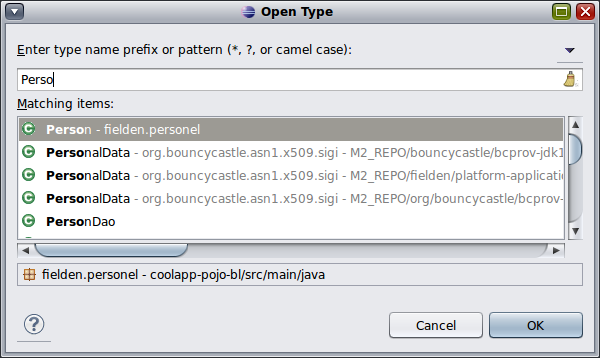
\includegraphics[width=0.6\textwidth]{parts/00-part/chapters/02-making-changes/images/01-open-type-person.png}
  \end{image}

  Open the type, make the changes in the code editor and save your them.
  In order to see the effect run the application from Eclipse IDE.
  This requires starting both the server (if it is not already running) and the client applications.
  The client application needs to be restarted is it was running at the time of changes in order to reload the recompiled classes.
  Although, the modified classes are shared between client and server applications, their reloading by the server is not essential as the performed changes effect only the client side.
  
  Once the client is up and running, go to \emph{Table Codes}$\longrightarrow$\emph{Personnel} and observer the affect of your changes, which should be obvious in the grid, selection criteria panel and in the configuration domain tree (can be invoked by clicking the \emph{Configure} button on Personnel Centre).
  
\subsection{Enhance Person and Test Your Changes}
  Let's now make some more serious changes. 
  
  \subsubsection*{The scenario.} 
  The following items should serve as a mini specification of the business rules for personnel enhancement.
  
  \begin{enumerate}
    \item Entity Person should be provided with a non-mandatory property \texttt{birthday}.
    \item This new property should be validated upon entry or change: 
	\begin{enumerate}
	  \item if the birth date value indicates that a person is too young (younger than 23 years of age) then a warning should be produced, but the value should be accepted;
	  \item no future birth dates should be accept.
	\end{enumerate}
  \end{enumerate}

  \subsubsection*{Implementing the requirements.}

  \paragraph*{Adding property.} 
  If the Eclipse IDE was property setup with TG templates, then creation of a new property is trivial.
  Type \texttt{tgp} and hit \texttt{Ctrl+Space} in the code editor of type Person under the last available property.
  This should result in the dialog depicted in Fig.~\ref{img:ch00:03:gen-prop-template}, which should be used to select option \texttt{tgprop} for property template generation.

  \begin{image}{TG Property Templates Dialog.}{\label{img:ch00:03:gen-prop-template}}
    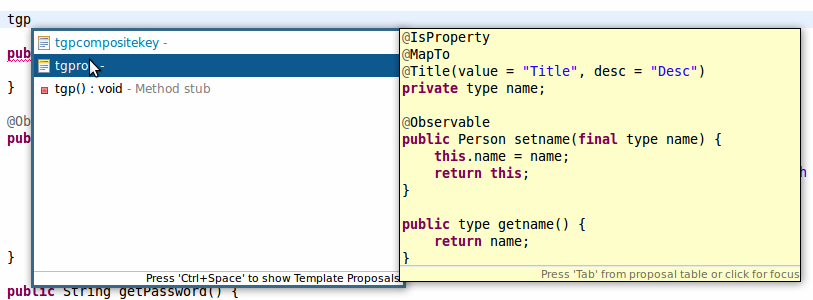
\includegraphics[width=0.8\textwidth]{parts/00-part/chapters/02-making-changes/images/02-birthday-property-gen.png}
  \end{image}

  The generation result is depicted in Fig.~\ref{img:ch00:03:prop-template}.
  Right after generation, the template is in edit mode, which means that all of its parts can be conveniently edited and navigated between using the \texttt{Tab} key.
  The first selected word is \emph{Title}, without moving the keyboard cursor or clicking anywhere with the mouse, start typing the new title \texttt{Birthday}.
  Hit the \texttt{Tab} key to move to the \texttt{desc} attribute and type \texttt{The date when person was born}.
  Hit the \texttt{Tab} key again to move to the \texttt{type} part and type \texttt{Date} to specify the property type.
  Hit the \texttt{Tab} key to move to the \texttt{name} and type \texttt{birthday} to give the property a field name.
  The next \texttt{Tab} will move the cursor to the setter name between the word \texttt{set} and \texttt{birthday}.
  Hit \texttt{Enter} to confirm changes.
  At this stage both setter and getter have the \texttt{birthday} portion starting with small \texttt{b}.
  Change it to be a capital \texttt{B}, so that the setter read \texttt{setBirthday} and getter read \texttt{getBirthday}.

  \begin{image}{TG Property Temple.}{\label{img:ch00:03:prop-template}}
    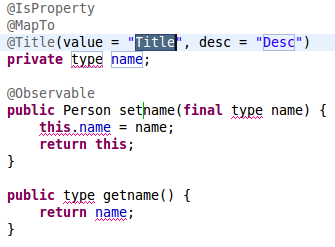
\includegraphics[width=0.4\textwidth]{parts/00-part/chapters/02-making-changes/images/03-birthday-property-template.png}
  \end{image}

  The final look of the property is provided in Listing~\ref{lst:Person-birthday}.
  Please note the return type of the setter, which matches the enclosing type Person.
  This is done to support method chaining, which is so convenient when creating new or modifying existing entity instances.

  \begin{code}{Property \texttt{birthday}.}{\label{lst:Person-birthday}}{codebgcolor}
    \begin{lstlisting}
    @IsProperty
    @MapTo
    @Title(value = "Birthday", desc = "The date when person was born")
    private Date birthday;
    
    @Observable
    public Person setBirthday(final Date birthday) {
      this.birthday = birthday;
      return this;
    }
    
    public Date getBirthday() {
      return birthday;
    }
    \end{lstlisting}
  \end{code}

  \paragraph*{Implementing validation.}
  The platform provides a sophisticated support for handling property before change events.
  This support, albeit in its simplest form, is demonstrated here for implementing birthday validation rules.

  First, annotate property \texttt{birthday} with \texttt{BeforeChange} as illustrated in Listing~\ref{lst:Person-birthday-beforechange} on line 3.
  The \texttt{Handler} is provided with value \texttt{BirthdayValidator.class}, which indicates the name of the wouldbe validator.
  This validator needs to be created.

  \begin{code}{BeforeChange declaration.}{\label{lst:Person-birthday-beforechange}}{codebgcolor}
    \begin{lstlisting}
    @IsProperty
    @MapTo
    @BeforeChange(@Handler(BirthdayValidator.class))
    @Title(value = "Birthday", desc = "The date when person was born")
    private Date birthday;
    \end{lstlisting}
  \end{code}

  Eclipse provides an easy way to generate the stub by clicking the error mark on the left margin of the editor and selecting option \emph{Create class 'BirthdayValidator'} as depicted in Fig.~\ref{img:ch00:03:gen-validator-class}.
  By default the invoked class\footnote{Please note that this time we're creating a new class that would provide the validation logic, but generally speaking it could also be an interface with customer specific binding that would happen at the project assembly phase.} creating wizard would offer to place it into the same package and the class where wizard was initiated.
  It is best if validators are kept in a separate to entities package in order to better organise the project structure.
  Thus, in the wizard change the package value from \texttt{fielden.personnel} to \texttt{fielden.personnel.validation}.

  \begin{image}{TG Property Temple}{\label{img:ch00:03:gen-validator-class}}
    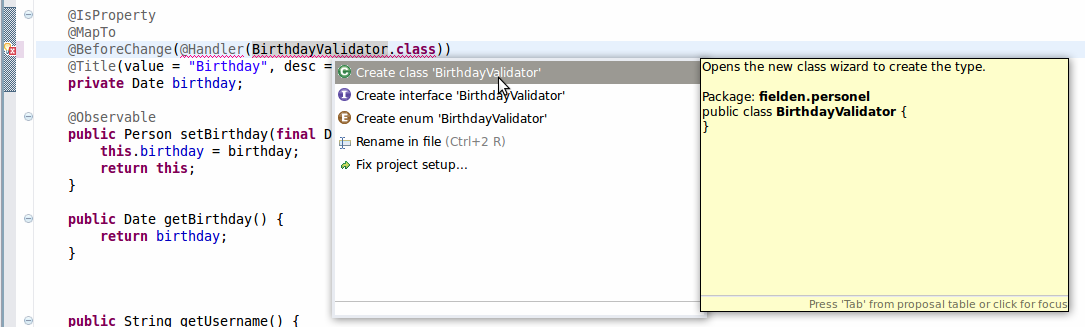
\includegraphics[width=\textwidth]{parts/00-part/chapters/02-making-changes/images/04-create-validator.png}
  \end{image}

  The generated class is an empty class, which does not explicitly extend any other class or implement any contracts\footnote{The term \emph{contract} is used in this book instead of the word \emph{interface} in order not to mix things up when taking about user interfaces and the interface, which is a contract that some class implements.}.
  In order for this class to become a proper \emph{before change event handler}, it needs to implement contract \texttt{IBeforeChangeEventHandler}, which requires one type parameter that should match the type of the property.
  In this case, it would be \texttt{Date} to match the type of property \texttt{birthday}.
  The contract demands implementation of only one method \texttt{handle} that would provide the necessary validation logic.
  
  The \emph{test-first} approach works really well when implementing business logic, which ensures both the correctness of the business logic and the quickest possible implementation time by navigating the development effort along the requirements captured by tests.
  Thus, let's first provide stub implementation for the handler class as illustrated in Listing~\ref{lst:Person-birthday-validation-stub}, and then implement the test that would define that should happen during birthday validation.  
  The stub returns a successful validation result, which is equivalent to not having any validation at all.
  
 \begin{code}{Birthday validation logic stub.}{\label{lst:Person-birthday-validation-stub}}{codebgcolor}
    \begin{lstlisting}
public class BirthdayValidator implements IBeforeChangeEventHandler<Date> {

    @Override
    public Result handle(final MetaProperty property, 
			 final Date newValue, final Date oldValue, 
			 final Set<Annotation> mutatorAnnotations) {
	return Result.successful(newValue);
    }
}
    \end{lstlisting}
  \end{code}
  
  The generated application conveniently provides an example of a domain-driven unit test case for entity Person.
  Open test case \texttt{PersonnelTest} by using the \emph{Open Type} dialog as before in the editor, and without explaining too much of the existing code\footnote{A separate chapter is dedicated to unit testing further in the book.} add the four tests from Listings~\ref{lst:Person-birthday-validation-test-1}-\ref{lst:Person-birthday-validation-test-4} to this test case.

  \begin{notebox}{A rule of thumb.}{\label{mb:rule-of-thumb}}
    Creation of unit tests should follow a rule of thumb where by \emph{each unit test should ensure one particular fact}.
    This keeps tests short in code and clear in meaning.
    The recommended approach is to use test method name to specify what fact it ensures.
    The provided examples follow this rule.
  \end{notebox}  

 \begin{code}{Personnel younger 23 should produce warning.}{\label{lst:Person-birthday-validation-test-1}}{codebgcolor}
    \begin{lstlisting}
@Test
public void birthday_indicating_a_young_person_should_produce_warning() {	
  final Person person = ao(Person.class).
			findByKey("USER2").
			setBirthday(new DateTime().minusYears(20).toDate());	

  assertTrue("Should be valid", 
             person.getProperty("birthday").isValid());
  assertNotNull("Should have warning", 
                person.getProperty("birthday").getFirstWarning());
}
    \end{lstlisting}
  \end{code}

\begin{code}{Personnel younger 23 should be persisted.}{\label{lst:Person-birthday-validation-test-2}}{codebgcolor}
    \begin{lstlisting}
@Test
public void birthday_indicating_a_young_person_should_be_saved() {	
  final Date birthday = new DateTime().minusYears(20).toDate();
  final Person person = ao(Person.class).
			findByKey("USER2").
			setBirthday(birthday);

  ao(Person.class).save(person);

  assertEquals("Incorrectly saved birthday.", 
	  birthday,
          ao(Person.class).findByKey("USER2").getBirthday());
}
    \end{lstlisting}
  \end{code}

  All tests rely on the fact that test data contains a person with business key equals to \emph{USER2} and property \texttt{birthday} that has no value (i.e. it is null).
  Test in Listing~\ref{lst:Person-birthday-validation-test-1} ensures rule \emph{2.a} that if the birth date suggests a person younger than 23 years of age then a warning should be raised, but the value should be recognised as valid.
  Test in Listing~\ref{lst:Person-birthday-validation-test-2} ensures that these ``early'' birthday value are saved correctly.
  Strictly speaking this test is not necessary and is provided only for the purpose of example, as it tests an already established at the platform level fact -- correct property values can be persisted when requested.

  The third test (Listing~\ref{lst:Person-birthday-validation-test-3}) ensures rule \emph{2.b} that no future birth dates are acceptable.
  The last test (Listing~\ref{lst:Person-birthday-validation-test-4}) ensures that invalid birthday value is not saved
  \footnote{Similar to test in Listing~\ref{lst:Person-birthday-validation-test-2}, it is provided more as an example -- the platform does not permit saving of invalid values, and there is no particular reason to test this invariant behaviour at the application level}.

\begin{code}{Unborn personnel should lead to a validation error.}{\label{lst:Person-birthday-validation-test-3}}{codebgcolor}
    \begin{lstlisting}
@Test
public void future_birthday_date_should_produce_validation_error() {	
  final Person person = ao(Person.class).
			findByKey("USER2").
			setBirthday(new DateTime().plusYears(1).toDate());	

  assertFalse("Should be invalid", 
              person.getProperty("birthday").isValid());
}
    \end{lstlisting}
  \end{code}

\begin{code}{Unborn personnel should not be persisted.}{\label{lst:Person-birthday-validation-test-4}}{codebgcolor}
    \begin{lstlisting}
@Test
public void future_birthday_date_should_not_be_saved() {	
  final Person person = ao(Person.class).
			findByKey("USER2").
			setBirthday(new DateTime().plusYears(1).toDate());	

  ao(Person.class).save(person);

  assertNull("Should have not been saved.", 
             ao(Person.class).findByKey("USER2").getBirthday());
}
    \end{lstlisting}
  \end{code}

  Running these tests by pressing \texttt{Ctrl+F11} combination while in the editor window of the test case, should result in failure of three out of four of the provided tests\footnote{The generated test \texttt{should\_be\_able\_to\_find\_person\_USER2} should also succeed.}.
  Test \texttt{birthday\_indicating\_a\_young\_person\_should\_be\_saved} succeeds because any value without validation is persisted when requested.
  For the same reason, test \texttt{future\_birthday\_date\_should\_not\_be\_saved} fails.

  The provided unit tests establish a set of constraints that guide the coding effort -- once all the tests pass the validation rule implementation can be declared completed.
  Listing~\ref{lst:Person-birthday-validation} provides a complete validation logic that satisfies all business requirements.
  Before moving further in the text please try to implement the validation rules personally without using code from the listing to make the tests pass.


 \begin{code}{Birthday validation logic}{\label{lst:Person-birthday-validation}}{codebgcolor}
    \begin{lstlisting}
public class BirthdayValidator implements IBeforeChangeEventHandler<Date> {

    @Override
    public Result handle(final MetaProperty property, 
			 final Date newValue, final Date oldValue, 
			 final Set<Annotation> mutatorAnnotations) {
	if (newValue != null) {
	    // let's use Joda Time for intermediate calculations
	    final DateTime date = new DateTime(newValue);
	    // reject future dates 
	    if (date.isAfterNow()) {
		return new Result(newValue, 
	                          new IllegalArgumentException("Cannot be in future."));
	    }
	    // warn if younger than 23 years of age 
	    if (date.isAfter(new DateTime().minusYears(23))) {
		return new Warning("The person is potentially too young.");
	    }
	}	
	
	return Result.successful(newValue);
    }
}
    \end{lstlisting}
  \end{code}

\subsection{Modifying User Interface}
  In order for application users to be able to enter and modify values of the \texttt{birthday} property added to the \emph{Person} entity, the application user interface (UI) needs to be updated.
  A complete discussion of the UI development support as provided by the platform is presented in chapter~\ref{?}.
  In this section we only cover the most essential concepts required to gain a general understanding in order to add \texttt{birthday} property to the application UI.

  The platform UI programming model is loosely based on a Model-View-Controller (MVC) pattern with stronger separation between the view and controller, which allows for a linear (instead of triad) dependency between the Model, View and Controller.
  Also, the nomenclature is slightly different:
  \begin{description}
    \item[\textbf{The View.}] Has the same meaning as in MVC, which is represented in TG by a specialised container (panel or frame) containing other UI controls. It is responsible strictly for layouting and holding UI controls and bares no UI logic.
    \item[\textbf{The Controller.}] Represents a pure business domain controller, which bares no UI logic\footnote{This separation of concerns is ensured at the module level, where business controller have no visibility of UI code.}. The View does not interact with Controller directly.
    \item [\textbf{The Model.}] Acts as a mediator between the View and Controller, and provides all UI related logic such as implementation of actions, event handlers etc. It interacts with Controller in order to invoke the business logic.
  \end{description}

  The basic modus operandi is this.
  Each domain entity such as \emph{Person} has a corresponding CRUD controller, UI model and view, which are bound together to enable user interaction with this domain entity.

 \begin{code}{Person main view construction}{\label{lst:Person-birthday-validation}}{codebgcolor}
    \begin{lstlisting}
@Override
public void buildUi() {
    final JPanel componentsPanel = new JPanel(new MigLayout("insets 0", 
					      "[:50:][grow, fill]", 
					      "[c]"));
    final Map<String, IPropertyEditor> editors = getModel().getEditors();
    ///////////////////////////////////////////////////////    
    addAndWrap(componentsPanel, editors, "key");  // row 1    
    addAndWrap(componentsPanel, editors, "desc"); // row 2
    ...
}
    \end{lstlisting}
  \end{code}


\subsection{Running Modified Application}

\subsection{Securing access}